\section{Auswertung}
	\label{sec:auswertung}

	\subsection{S"attigungsstr"ome und Kennlinien der Hochvakuumdiode}
		Um den S"attigungsstrom $I_\mathrm{s}$ der Diode abzusch"atzen, werden f"ur f"unf Heizstromst"arken $I_\mathrm{H}$ die Kennlinien aufgetragen.
		Hierf"ur wird der Diodenstrom $I$ gegen das Diodenpotential $U$ aufgetragen.
		F"ur Str"ome $I > \SI{1.25}{\milli \ampere}$ zeigt das Strommessger"at eine "Uberlastung an.
		Weil dieser Wert jedoch bei den Heizstromst"arken $I_\mathrm{H} = \SI{2.9}{\ampere}$ und $I_\mathrm{H} = \SI{3.1}{\ampere}$ erreicht wird, bevor ein Abflachen der Kurve erkannt werden kann, k"onnen lediglich drei S"attigungsstr"ome abgelesen werden:

		\begin{eqnarray*}
			I_\mathrm{H} = \SI{2}{\ampere}, \, U_\mathrm{H} = \SI{3}{\volt} & \Rightarrow & I_{\mathrm{s},1} = \SI{4}{\nano \ampere}\, \\
			I_\mathrm{H} = \SI{2.3}{\ampere}, \, U_\mathrm{H} = \SI{3.5}{\volt} & \Rightarrow & I_{\mathrm{s},2} = \SI{40}{\nano \ampere}\, \\
			I_\mathrm{H} = \SI{2.6}{\ampere}, \, U_\mathrm{H} = \SI{4}{\volt} & \Rightarrow & I_{\mathrm{s},3} = \SI{.32}{\milli \ampere}\, \\
		\end{eqnarray*}

		Die Folgenden zwei Graphen visualisieren die Messdaten, sowie die gesch"atzten S"attigungsstr"ome $I_\mathrm{s}$.
		Die Messdaten sind anschlie"sen in Tabelle \ref{messung1} aufgef"uhrt.

		\clearpage

		\begin{figure}[h!]
			\centering
			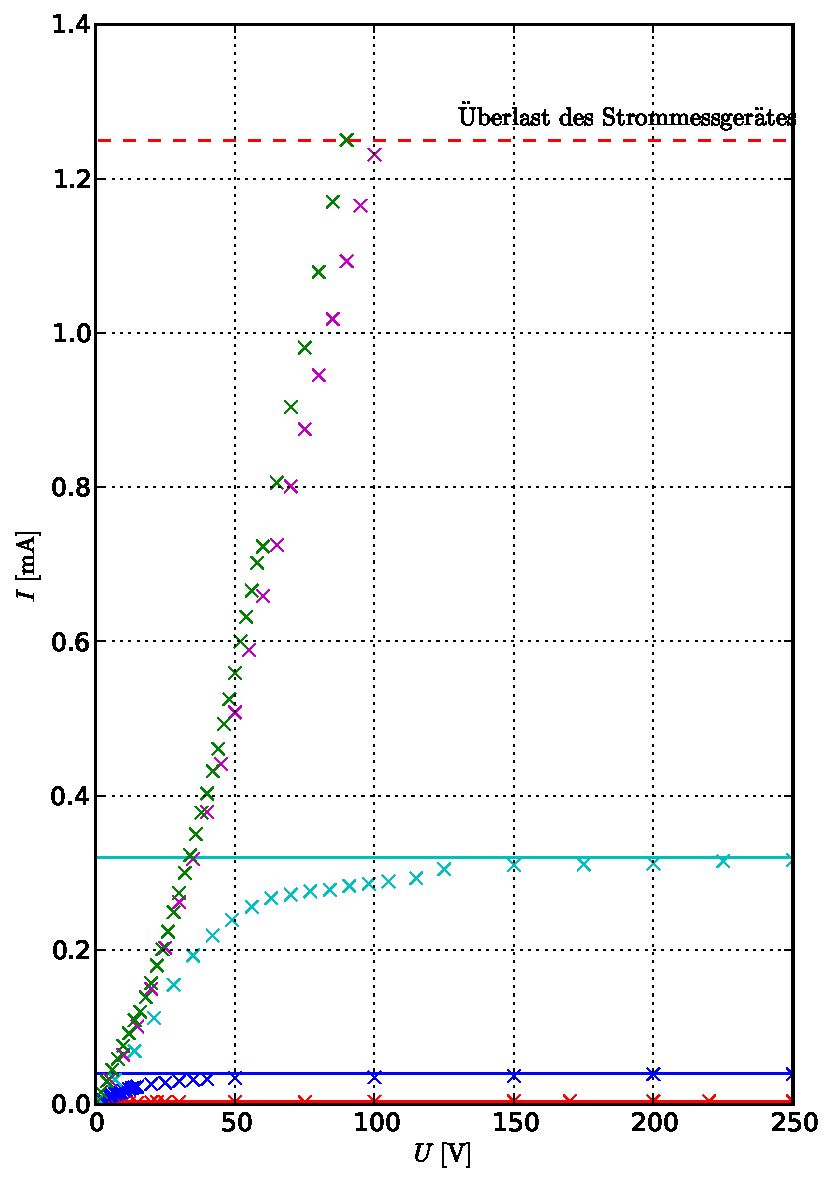
\includegraphics[width = 15cm]{img/kennlinie1.pdf}
			\caption{Kennlinien der Hochvakuumdiode f"ur Heizstr"ome von $I_\mathrm{s} = \SI{2}{\ampere}$ bis $I_\mathrm{s} = \SI{3.1}{\ampere}$.}
			\label{fig:kennlinie1}
		\end{figure}

		\begin{figure}[h!]
			\centering
			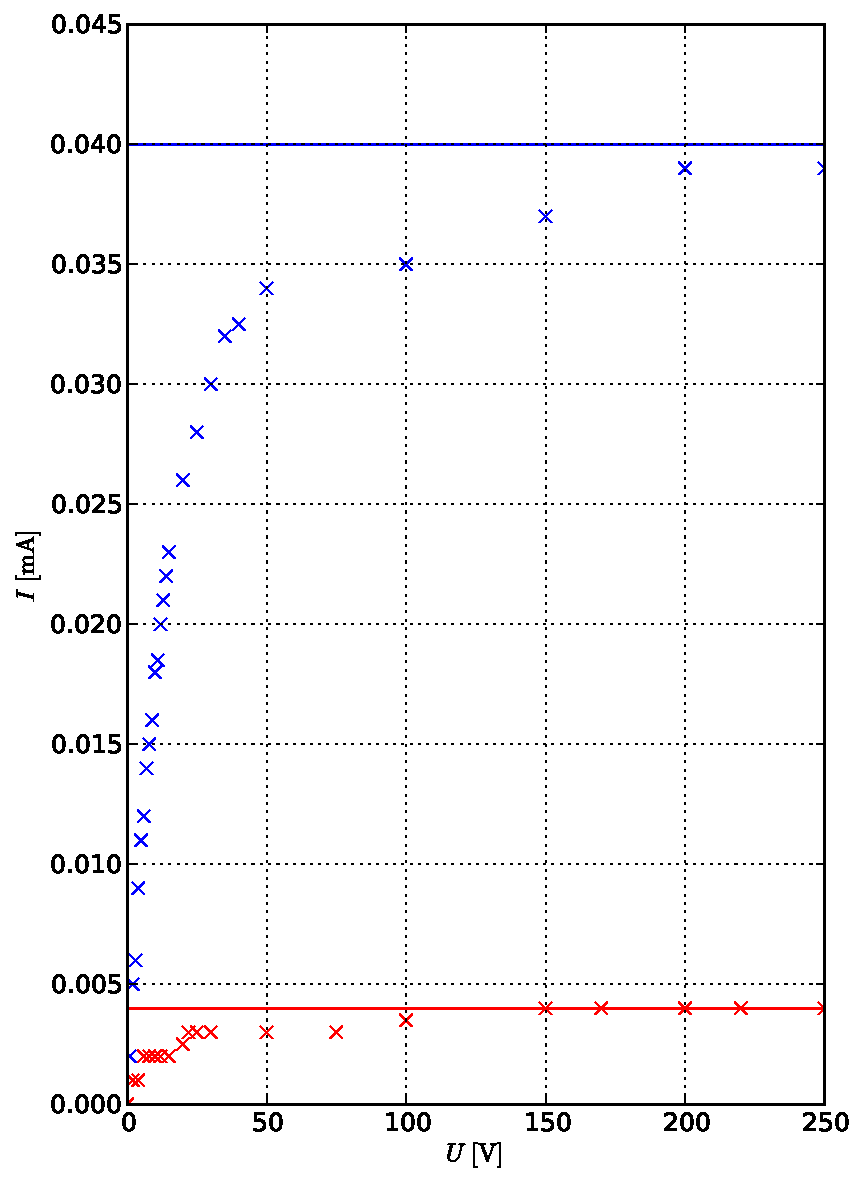
\includegraphics[width = 15cm]{img/kennlinie2.pdf}
			\caption{Kennlinien der Hochvakuumdiode f"ur Heizstr"ome von $I_\mathrm{s} = \SI{2}{\ampere}$ und $I_\mathrm{s} = \SI{2.3}{\ampere}$. In dieser Aufl"osung lassen sich die Werte besser erkennen.}
			\label{fig:kennlinie2}
		\end{figure}

		\clearpage

		\begin{table}[h!]
			\begin{center}
				\label{messung1}
				\caption{Messwerte f"ur die Diodenkennlinien. F"ur die Verifizierung des Langmuir-Schottkyschen Raumladungsgesetzes wurden bei maximaler Heizleistung besonders viele Messwerte genommen.}
				\begin{tabular}{|r|r||r|r||r|r||r|r||r|r|}
					\hline
						\multicolumn{2}{|c||}{$I_\mathrm{H} = \SI{2}{\ampere}$} &
						\multicolumn{2}{c||}{$I_\mathrm{H} = \SI{2.3}{\ampere}$} &
						\multicolumn{2}{c||}{$I_\mathrm{H} = \SI{2.6}{\ampere}$} &
						\multicolumn{2}{c||}{$I_\mathrm{H} = \SI{2.9}{\ampere}$} &
						\multicolumn{2}{c|}{$I_\mathrm{H} = \SI{3.1}{\ampere}$} \\
						\multicolumn{2}{|c||}{$U_\mathrm{H} = \SI{3}{\ampere}$} &
						\multicolumn{2}{c||}{$U_\mathrm{H} = \SI{3.5}{\ampere}$} &
						\multicolumn{2}{c||}{$U_\mathrm{H} = \SI{4}{\ampere}$} &
						\multicolumn{2}{c||}{$U_\mathrm{H} = \SI{5}{\ampere}$} &
						\multicolumn{2}{c|}{$U_\mathrm{H} = \SI{6}{\ampere}$} \\
					\hline 
						$U$ [V] & $I$ [mA] & $U$ [V] & $I$ [mA] & $U$ [V] & $I$ [mA] & $U$ [V] & $I$ [mA] & $U$ [V] & $I$ [mA] \\
					\hline 
					\hline
						0      &   0 & 0,0020 &   1 & 0,006 & 001 & 0,032 & 005 &  0 & 0,001 \\
0,001  &   2 & 0,0050 &   2 & 0,032 & 007 & 0,064 &	010 &  2 & 0,016 \\
0,001  &   4 & 0,0060 &   3 & 0,069 & 014 & 0,101 &	015 &  4 & 0,030 \\
0,002  &   6 & 0,0090 &   4 & 0,112 & 021 & 0,150 &	020 &  6 & 0,045 \\
0,002  &   8 & 0,0110 &   5 & 0,155 & 028 & 0,203 &	025 &  8 & 0,059 \\
0,002  &  10 & 0,0120 &   6 & 0,193 & 035 & 0,262 &	030 & 10 & 0,076 \\
0,002  &  12 & 0,0140 &   7 & 0,219 & 042 & 0,318 &	035 & 12 & 0,092 \\
0,002  &  15 & 0,0150 &   8 & 0,239 & 049 & 0,379 &	040 & 14 & 0,109 \\
0,0025 &  20 & 0,0160 &   9 & 0,256 & 056 & 0,441 &	045 & 16 & 0,120 \\
0,003  &  22 & 0,0180 &  10 & 0,267 & 063 & 0,508 &	050 & 18 & 0,139 \\
0,003  &  25 & 0,0185 &  11 & 0,272 & 070 & 0,589 &	055 & 20 & 0,157 \\
0,003  &  30 & 0,0200 &  12 & 0,276 & 077 & 0,659 &	060 & 22 & 0,180 \\
0,003  &  50 & 0,0210 &  13 & 0,278 & 084 & 0,725 &	065 & 24 & 0,201 \\
0,003  &  75 & 0,0220 &  14 & 0,283 & 091 & 0,801 &	070 & 26 & 0,224 \\
0,0035 & 100 & 0,0230 &  15 & 0,286 & 098 & 0,875 &	075 & 28 & 0,249 \\
0,004  & 150 & 0,0260 &  20 & 0,305 & 125 & 0,945 &	080 & 30 & 0,274 \\
0,004  & 170 & 0,0280 &  25 & 0,310 & 150 & 1,018 &	085 & 32 & 0,300 \\
0,004  & 200 & 0,0300 &  30 & 0,311 & 175 & 1,093 &	090 & 34 & 0,323 \\
0,004  & 220 & 0,0320 &  35 & 0,312 & 200 & 1,165 &	095 & 36 & 0,350 \\
0,004  & 250 & 0,0325 &  40 & 0,315 & 225 & 1,231 &	100 & 38 & 0,378 \\
       &     & 0,0340 &  50 & 0,317 & 250 &	      &     & 40 & 0,403 \\
       &     & 0,0350 & 100 & 0,289 & 105 &	      &     & 42 & 0,432 \\
       &     & 0,0370 & 150 & 0,293 & 115 &	      &     & 44 & 0,461 \\
       &     & 0,0390 & 200 &       &     &       &     & 46 & 0,493 \\
       &     & 0,0390 & 250 &       &     &       &     & 48 & 0,525 \\
       &     &        &     &       &     &       &     & 50 & 0,559 \\
       &     &        &     &       &     &       &     & 52 & 0,600 \\
       &     &        &     &       &     &       &     & 54 & 0,632 \\
       &     &        &     &       &     &       &     & 56 & 0,666 \\
       &     &        &     &       &     &       &     & 58 & 0,702 \\
       &     &        &     &       &     &       &     & 60 & 0,723 \\
       &     &        &     &       &     &       &     & 65 & 0,806 \\
       &     &        &     &       &     &       &     & 70 & 0,904 \\
       &     &        &     &       &     &       &     & 75 & 0,981 \\
       &     &        &     &       &     &       &     & 80 & 1,079 \\
       &     &        &     &       &     &       &     & 85 & 1,170 \\
       &     &        &     &       &     &       &     & 90 & 1,250 \\
					\hline 
				\end{tabular}
			\end{center}
		\end{table}

		\clearpage

	\subsection{Verifizierung des Langmuir-Schottkyschen Raumladungsgesetzes}
		\label{subsec:langmuir}
		Um die Vorhersage des Langmuir-Schottkyschen Raumladungsgesetzes zu pr"ufen, wurden bei maximalem Heizstrom $I_\mathrm{H} = \SI{3.1}{\ampere}$ m"oglichst viele Werte aufgenommen.
		Das Gesetz gilt in einem Bereich von $U = 0$ bis zum Wendepunkt der Diodenkennlinie.
		Weil in dieser Messreihe kein Wendepunkt erkennbar ist wird angenommen, dass das Gesetz f"ur alle Werte erf"ullt ist.

		Es gilt dann

		\begin{eqnarray*}
			I & \propto & U^a\,, \\
			\Leftrightarrow \quad \ln{I} & \propto & a \ln{U}\,.
		\end{eqnarray*}

		Mit einem Konstanten Exponenten $a$, der durch lineare Regression ermittelt werden kann und etwa den Wert $a_\mathrm{Theorie} = 3/2$ annehmen sollte.

		Lineare Regression mit Hilfe des Python-Moduls numpy ergibt

		\begin{equation*}
			a = \SI{1.204 (7)}{}\,.
		\end{equation*}

		Zus"atzlich wird eine nicht-lineare Regression durch numpy durchgef"uhrt und liefert

		\begin{equation*}
			a = \SI{1.380 (8)}{}\,.
		\end{equation*}

		\clearpage

		\begin{figure}[h]
			\centering
			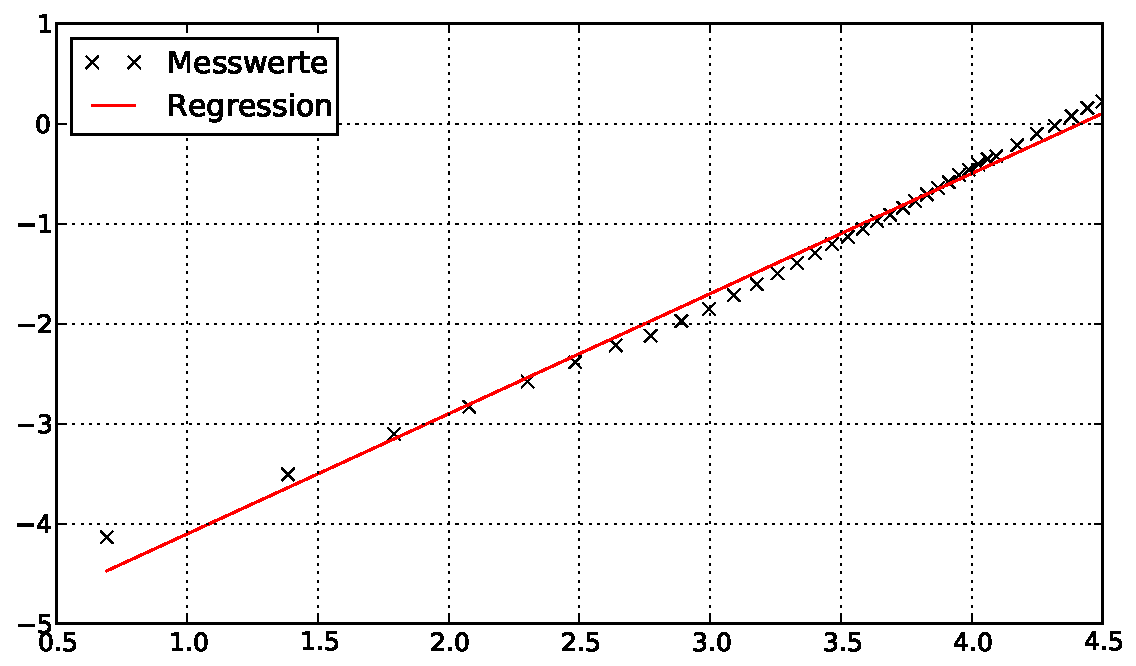
\includegraphics[width = 10cm]{img/langmuir.pdf}
			\caption{Lineare Regression der $(\ln{U},\ln{I})$ Wertepaare zur kontrolle des Exponenten des Langmuir-Schottkyschen Raumladungsgesetzes.}
			\label{fig:langmuir}
		\end{figure}

		\begin{figure}[h]
			\centering
			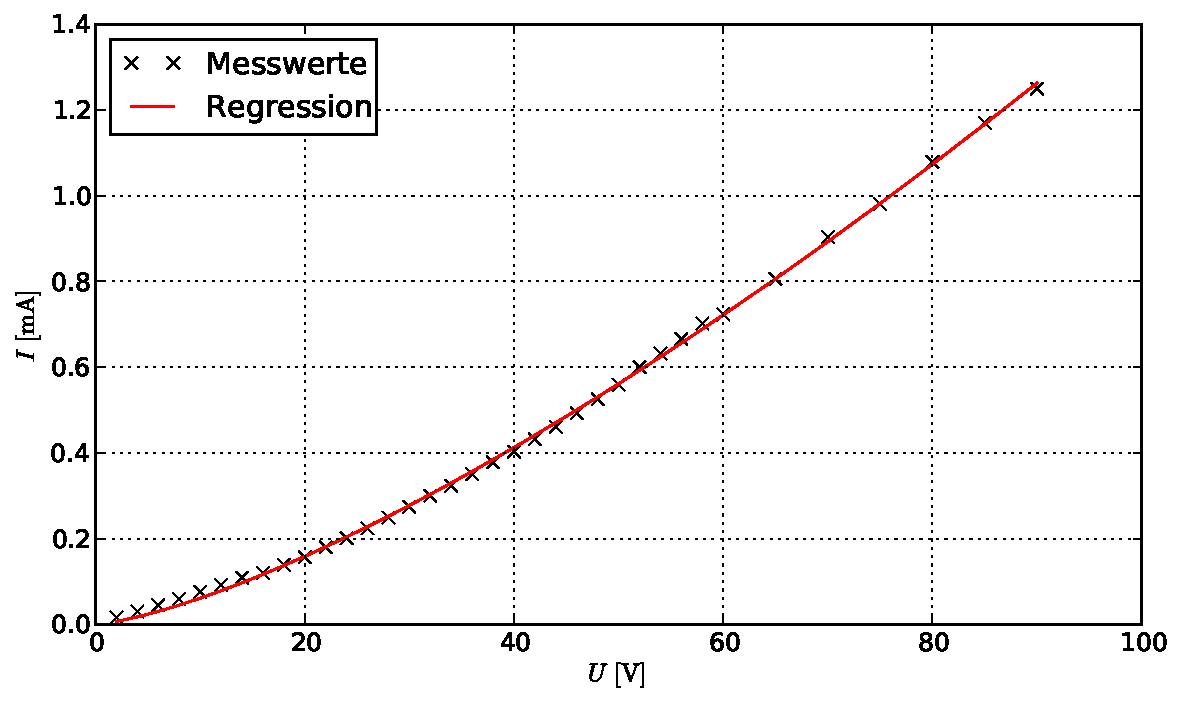
\includegraphics[width = 10cm]{img/langmuir_nichtlinear.pdf}
			\caption{Nicht-lineare Regression der $(U,I)$ Wertepaare zur kontrolle des Exponenten des Langmuir-Schottkyschen Raumladungsgesetzes.}
			\label{fig:langmuir_nichtlinear}
		\end{figure}

		\enlargethispage{10cm}

		\clearpage

	\subsection{Bestimmung der Kathodentemperatur...}
		\subsubsection{...mit Hilfe des Kathodenstromes $I$ und der Kathodenspannung $U$ im Anlaufstromgebiet}
			\label{subsubsec:temp1}
			Aus den Wertepaaren $(U,I)$ im Anlaufstromgebiet der Diode bei maximaler Heizleistung ($I_\mathrm{H} = \SI{3.1}{\ampere}$), l"asst sich die Temperatur $T$ der Kathode ermitteln.
			Wegen der Beziehung

			\begin{equation*}
				I(U) \propto \exp{\left(-\frac{e_0 U}{kT}\right)}
			\end{equation*}

			l"asst sich T durch lineare Regression von $\ln{I}$ gegen $c\cdot U$ bestimmen. Die Berechnung durch numpy liefert dann denn Wert f"ur $c$, woraus sich $T$ errechnen l"asst.
			Es ist zu beachten, dass die gemessene Spannung $U$ um die im Messger"at abfallenden Spannung $U_- = I \cdot \SI{1}{\mega \ohm}$ korrigiert werden muss.
			Die Regression wird also mit $U_\mathrm{k} = U - U_-$ durchgef"uhrt.

			Die Temperatur $T$ ist dabei au"serdem mit einem Fehler behaftet der mittels Gau"sscher Fehlerfortpflanzung bestimmt wird.
			Es gilt

			\begin{eqnarray*}
				c & = & -\frac{e_0}{kT}\,\\
				\Leftrightarrow \quad T & = & -\frac{e_0}{kc}\,,\\
				\Delta T & = & \frac{e_0}{kc^2}\Delta c\,,
			\end{eqnarray*}

			mit der Stefan-Boltzmann Konstante $k = \SI{1.381e-23}{\joule \per \kelvin}$ \cite{nist} und der Elementarladung $e_0 = \SI{1.602e-19}{\coulomb}$ \cite{nist}.

			Die Regression liefert

			\begin{eqnarray*}
				c & = & \SI{-3.360 (88)}{\coulomb \per \joule}\,\\
				\Rightarrow \quad T & = & \SI{3454 (90)}{\kelvin}\,.
			\end{eqnarray*}

			\begin{figure}[h!]
				\centering
				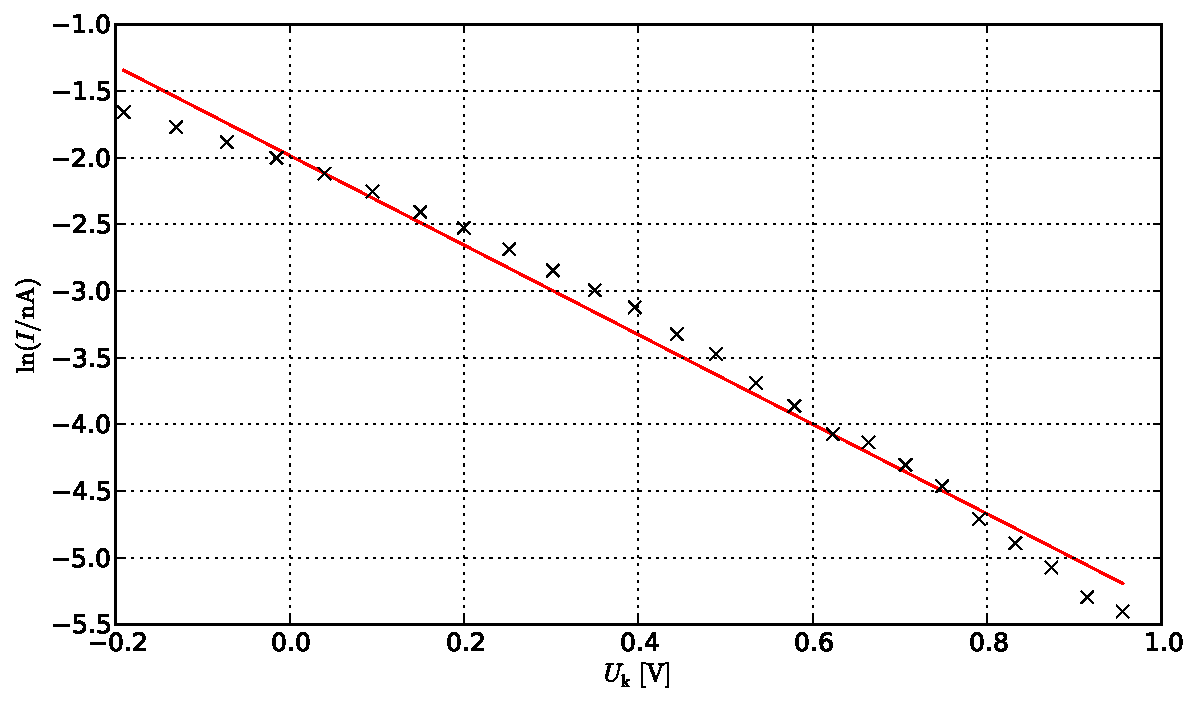
\includegraphics[width = 15cm]{img/messung2.pdf}
				\caption{Lineare Regression von $\ln{I}$ gegen $U_\mathrm{k}$ im Anlaufstrombereich.}
				\label{fig:messung2}
			\end{figure}

			\begin{table}[h!]
				\begin{center}
					\label{messung1}
					\caption{Messwerte f"ur Diodenspannung $U$, $U_\mathrm{k}$ und -strom $I$ im Anlaufstrombereich.}
					\begin{tabular}{|r|r|r||r|r|r|}
						\hline
							$U$ [V] & $U_\mathrm{k}$ [V] & $I$ [mA] & $U$ [V] & $U_\mathrm{k}$ [V] & $I$ [mA] \\
						\hline 
						\hline
							0,0& -0,19 &	0,19&	0,52 & 0,489 &	0,031\\
0,04 & -0,13 &	0,17&	0,56 & 0,535 &	0,025\\
0,08 & -0,072 &	0,152&	0,6& 0,579 &	0,021\\
0,12 & -0,015 &	0,135&	0,64 & 0,623 &	0,017\\
0,16 & 0,04 &	0,12&	0,68 & 0,664 &	0,016\\
0,2& 0,095 &	0,105&	0,72 & 0,7065 &	0,0135\\
0,24 & 0,15 &	0,09&	0,76 & 0,7485 &	0,0115\\
0,28 & 0,2 &	0,08&	0,8& 0,791 &	0,009\\
0,32 & 0,252 &	0,068&	0,84 & 0,8325 &	0,0075\\
0,36 & 0,302 &	0,058&	0,88 & 0,87375 &	0,00625 \\
0,4& 0,35 &	0,05&	0,92 & 0,915 &	0,005\\
0,44 & 0,396 &	0,044&	0,96 & 0,9555 &	0,0045\\
0,48 & 0,444 &	0,036&		 &		&	\\



























						\hline 
					\end{tabular}
				\end{center}
			\end{table}

			\clearpage

		\subsubsection{...mit Hilfe der Heizleistung $U_\mathrm{H}I_\mathrm{H}$}
			\label{subsubsec:temp2}
			Anhand der Heizleistung $U_\mathrm{H}I_\mathrm{H}$ der Kathodenheizung l"asst sicht die Temperatur $T$ der Kathode ebenfalls bestimmen.
			Es gilt dabei

			\begin{equation*}
				T = \left(\frac{I_\mathrm{H}U_\mathrm{H} - N_\mathrm{WL}}{f \eta \sigma}\right)^{\frac{1}{4}}\,,
			\end{equation*}

			mit der Stefan-Boltzmannschen Strahlungskonstante $\sigma = \SI{5.670e-8}{\watt \per \meter \squared \per \kelvin \tothe{4}}$ \cite{nist}, der Kathodenoberfl"ache $f = \SI{.35}{\centi \meter \squared}$ \cite{anleitung}, dem Emissionsgrad $\eta = \SI{.28}{}$ \cite{nist} und der W"armeleitung $N_\mathrm{WL} = \SI{.9}{}$ \cite{nist}.
			Wegen Ablesefehlern des Heizstromes $I_\mathrm{H}$ und der Heizspannung $U_\mathrm{H}$ ist die Temperatur $T$ fehlerbehaftet.
			F"ur den Fehler gilt nach Gau"sscher Fehlerfortpflanzung

			\begin{equation*}
				\Delta T = \frac{1}{4} \left(f\eta \sigma\right)^{-\frac{1}{4}} \left| I_\mathrm{H}U_\mathrm{H} - N_\mathrm{WL} \right|^{-\frac{3}{4}} \left(U_\mathrm{H} \Delta I_\mathrm{H} + I_\mathrm{H} \Delta U_\mathrm{H} \right)\,.
			\end{equation*}

			Damit ergeben sich die Werte
			\begin{table}[h!]
				\begin{center}
					\label{messung1}
					%\caption{Messwerte f"ur Diodenspannung und -strom im Anlaufstrombereich.}
					\begin{tabular}{|r|r|r|}
						\hline
							$I_\mathrm{H}$ [A] & $U_\mathrm{H}$ [V] & $T$ [K] \\
							\pm 0,1\,A&\pm 0,1\,V & \\ 
						\hline 
						\hline
							2,0 & 3,0 & $\SI{1741 (4)}{}$ \\
							2,3 & 3,5 & $\SI{1894 (4)}{}$ \\
							2,6 & 4,0 & $\SI{2033 (4)}{}$ \\
							2,9 & 5,0 & $\SI{2224 (3)}{}$ \\
							3,1 & 6,0 & $\SI{2376 (3)}{}$ \\
						\hline 
					\end{tabular}
				\end{center}
			\end{table}

	\subsection{Bestimmung der Austrittsarbeit}
		\label{subsec:austrittsarbeit}
		Mit Hilfe der Richardson-Gleichung l"asst sich schlie"slich aus den S"attigungsstr"omen $I_\mathrm{s}$ die Austrittsarbeit von Elektronen im gegebenen Material bestimmen.
		Es gilt

		\begin{eqnarray*}
			e_0 \Phi & = & -kT \cdot \ln{\left( \frac{I_\mathrm{s} h^3}{4 \pi e_0 m_0 k^2 T^2} \right)}\,, \\
			\Delta e_0 \Phi & = & \left| k \ln \left( \frac{I_\mathrm{s} h^3}{4 \pi e_0 m_0 k^2 T^2} \right) \right| \Delta T \,.
		\end{eqnarray*}

		Hier bezeichnet $h = \SI{6.626e-34}{\joule \second}$ \cite{nist} das Plancksche Wirkungsquantum und $m_0 = \SI{9.109e-31}{\kilo \gram}$ \cite{nist} die Elektronenmasse.

		\clearpage

		Man erh"alt

		\begin{table}[h!]
			\begin{center}
				\label{messung1}
				%\caption{Messwerte f"ur Diodenspannung und -strom im Anlaufstrombereich.}
				\begin{tabular}{|r|r|r|}
					\hline
						$I_\mathrm{s}$ [nA] & $T$ [K] & $e_0 \Phi$ [eV] \\
					\hline 
					\hline
						4 & $\SI{1741 (4)}{}$ & $\SI{7.240 (2)}{}$\\
						40 & $\SI{1894 (4)}{}$ & $\SI{5.649 (2)}{}$ \\
						320 & $\SI{2033 (4)}{}$ & $\SI{7.741 (2)}{}$ \\
					\hline 
				\end{tabular}
			\end{center}
		\end{table}

		Durch Bildung des Mittelwertes "uber alle $n = 3$ Werte und des Fehlers

		\begin{equation*}
			\Delta x = \left(\sum_{i=1}^{n} (\Delta x_i)^2\right)^{\frac{1}{2}}\,,
		\end{equation*}

		erh"alt man f"ur die Austrittsarbeit:

		\begin{eqnarray*}
			\overline{e_0 \Phi} = \SI{6.877 (3)}{\electronvolt}\,.
		\end{eqnarray*}

